\documentclass{article}
\usepackage[utf8]{inputenc}

\usepackage{amsmath}
\usepackage{amssymb}
\usepackage{booktabs}

\usepackage[authoryear]{natbib}
\renewcommand{\bibname}{References}

% \usepackage{float}
\usepackage{floatrow}
\newfloatcommand{capbtabbox}{table}[][\FBwidth]

\usepackage[bb=dsserif]{mathalpha}
\usepackage{bm}
\usepackage{graphicx}
\usepackage{eucal}
\usepackage{caption}
\usepackage{subcaption}
\usepackage{titlesec}
\usepackage{comment}
\captionsetup[table]{labelfont={bf,large},textfont={bf,large},justification=centering}
\captionsetup[figure]{labelfont={bf,normalsize},textfont={bf,normalsize},justification=centering}
\usepackage{float}
\usepackage{geometry}
 \geometry{
 a4paper %,
%  total={170mm,257mm} %,
%  left=20mm,
%  top=20mm,
 }

\title{Identifying Average Firm and Worker Effects in Matched Employer-Employee Data: A Research Proposal}
\author{Nathan Lazarus}
\date{April 5, 2022}

\begin{document}
\bibliographystyle{ecta}
\clearpage\maketitle
\thispagestyle{empty}

\begin{abstract}
    I show that, even with the assumptions required for them to have a causal interpretation, high dimensional fixed effects estimators, do not recover the average effects of firms or workers on wages if there is heterogeneity or dynamic effects of either firms or workers on wages. This is well-known in the context of differences-in-differences estimation, where two-way fixed effects (TWFE) models do not identify the causal estimands that are typically of interest. Here, I point out that these issues extend to high-dimensional fixed effects estimation, and that these biases are salient in the context of labor economics. Heterogeneous treatment effects correspond to match effects between firms and workers and dynamic treatment effects correspond to firm- and worker-specific tenure-earnings profiles. Typical estimation of match effects in an AKM model \citep{woodcock2015match} rely on TWFE estimation that does not identify the average effect in the presence of match effects. I define a notion of average effects that is relevant here, show examples of the bias of TWFE relative to this notion of average effects, and sketch an alternative estimator. The estimator I propose cannot be implemented, and it's not clear that it would identify the average effect even if it could be. I hope to extend this work to find a better estimator, as well as to implement it on matched employer-employee data and test whether it makes a substantial difference in the conclusions relative to previous work.
\end{abstract}



% Oftentimes, especially in research on firms and workers, economists are interested in high-dimensional fixed effects estimators that recover the effects of firm and worker components of wages. With additional assumptions (exogenous mobility) these effects can be interpreted as causal effects of changing firms on worker wages and the causal effects of changing workers on firm wages. 

% I show that in high-dimensional fixed effects models, if the fixed effects have a causal interpretation, they do not correspond to the average treatment effect in the cases of dynamic or heterogenous treatment effects or heterogeneous effects of covariates. Instead, they correspond to a weighted average of the causal effects of, say, a given firm on its worker's wages (treatment on the treated), where the weights can be negative. This is well-known in the context of differences-in-differences estimation, where two-way fixed effects models do not identify the causal estimands that are typically of interest. Here, I point out that these issues extend to fixed effects, and that these biases are salient in the context of labor economics. Heterogeneous treatment effects correspond to match effects between firms and workers, dynamic treatment effects correspond to firm- and worker-specific tenure-earnings profiles, and heterogeneous effects of covariates correspond to heterogeneous age-earnings profiles when age is included as a covariate. I show examples where a firm has strictly positive causal effects on worker wages, but is estimated to have a negative fixed effect. I then outline an alternative estimator of the average effects of firms on their workers' wages and the average effects of workers' on the wages they receive (corresponding to the ATT), and . I hope to extend this work to estimate the effects on matched employer-employee data and provide alternative computationally tractable estimators.\\
\setcounter{page}{0}

\newpage

\section{Overview}

% I propose ... 
Suppose a researcher observes two firms, who are matched with two workers over the course of a panel. The researcher can label the firms $1$ and $0$, and regress wages on firm, with worker and time fixed effects, to estimate the effect of firms on earnings (provided that all four matches are observed). Similarly, one can regress wages on worker with firm and time fixed effects, and recover the worker effects. These firm and worker fixed effects are of interest in a large body of literature that seeks to understand the extent of assortative matching in the labor market going back to \citet*{abowd1999high} (AKM), as well as a wide variety of other work that tries to understand whether differences in worker-firm matches can explain various dimensions of inequality. Here, I make the analogy with differences-in-differences estimation, where $0$ and $1$ correspond to the treated and untreated states.

In differences-in-differences, the object of interest is typically the average treatment on the treated (ATT). Below, I discuss the analog of that for AKM (the average firm and worker effect in realized matches). Many estimators for this average treatment on the treated are possible, but the most common one in differences-in-differences estimation until recently was the two-way fixed effects (TWFE) regression specification, that controlled for unit and time fixed effects. In a number of cases, these TWFE specifications fail to identify the ATT, as shown by \citet{borusyak2021revisiting}. AKM estimates of firm and worker effects also are typically estimated with a two-way fixed effects design, and are therefore subject to the same issues identified by Borusyak et al.

A number of other estimators have been proposed recently in this staggered differences-in-differences context to recover the average treatment effect on the treated of a binary treatment on a continuous outcome with unit and time fixed effects. These estimators recover the ATT even in the presence of heterogeneity in treatment effects across units, time, and event time. The AKM setting is more challenging because instead of a binary treatment, we want to identify the average treatment effects of a multivalued categorical treatment (firm or worker). In addition, AKM, in the above interpretation, implements two separate regressions: wages on firm with worker and time fixed effects, and wages on worker with firm and worker fixed effects. In the two-way fixed effects setup, it's unnecessary to run two regressions---the fixed effects from one regression are the ``treatment effect'' estimates from the other, and under the additive model they both correspond to the average treatment effect. But the differences-in-differences estimators choose which comparisons to make based on treatment status, and therefore do not treat treatment variables and control fixed effects the same way. Additionally, most of the differences-in-differences estimators focus on the setting in which treatment is an absorbing state, so there would be transitions from firm 0 to firm 1 but none in the other direction, which is not the case. So the differences-in-differences literature gives a guide for robust estimation of the average firm effect in the case of two firms, unidirectional flows, and constant worker effects.

I am working on %propose to attempt to figure out?
an estimator that recovers the average firm and worker effects in the presence of unit and event time heterogeneity. These are important quantities in labor economics: heterogeneity in firm effects across workers or worker effects across firms means that there are match effects. In the case of perfect competition (where firm effects are 0), match effects would mean that workers are differentially productive at different firms, which is a natural consequence of differential production technology and skills, as in \citet{roy1951some}. But there has been a particular interest recently in understanding imperfectly competitive labor markets with AKM (\citealp{card2018firms}, \citealp{lamadon2022imperfect}). If imperfect competition is rationalized with differential tastes of workers for firms, due to idiosyncratic preferences for firm-specific amenities, then tastes and productivity can determine matched wages. Workers demand a higher wage to work at a firm with amenities they desire less.\footnote{In the competitive case, the worker is paid their marginal product at any firm, so if we considered an off-equilibrium match where the worker has very low productivity, that would imply a very low, but clearly defined, wage. But in the monopsonistic case, at on off-equilibrium match, the worker's amenity value could be very low, so their reservation wage would be high, and their productivity could be low, so there needs to be a splitting rule for the negative joint surplus to pin down the counterfactual wage.}
% So at the off-equilibrium firms, the firm's willingness to pay could be lower (because the worker lacks the appropriate skills) while the worker's reservation wage could be higher (because of lower amenity values), and the overall match surplus can be negative. That is why those matches don't occur in equilibrium! But in terms of the notion of average treatment on the treated, those matches are in the comparison group and there has to be some way of pinning down those counterfactual wages.

Event time heterogeneity is also interesting in the context of labor economics. This means that there are firm- or worker-specific tenure-earnings profiles. This sort of heterogeneity emerges if different firms would offer a different schedule of raises to the same worker, which seems quite natural. This could be because workers experience different productivity growth at different firms because some firms are better learning environments (\citealp{jarosch2021learning}, \citealp{gregory2020firms}), or it could be just because of idiosyncratic choices of firms as to when they offer raises, say every year or every other year. Similarly, worker-specific tenure-earnings profiles could emerge if some workers acquire firm-specific human capital more quickly than other workers.

These issues are specific to the problem of identifying the ATT. If one is simply interested in any weighted combination of treatment effects, TWFE identifies some such combination. The TWFE weights will have large impacts on the relative variance of the firm and worker effects.\footnote{It is clear to me in simulations that the fixed effects are very volatile in simulations even when the average effect remains constant, but I haven't done the variance decomposition yet to formally show this.} In these contexts, I claim that the ATT is the most interesting and natural object to work with. Here, the firm effect of firm $1$ is the average difference between the wage that it pays its workers and the wage that those workers would receive at other firms. Similarly, the worker effect is the difference between the wage at the firm that workers are observed matched to (in a given year) and the average wage that other workers would have received if matched to that firm. %complication: multiple workers can be matched to a firm: do colleagues go in the counterfactual?

These ATTs are causal objects. Given that AKM is typically estimated on observational data, some work focuses more on interpreting it as an interesting decomposition of realized wages, while recognizing that it can be confounded by things like differences between the realized wages of movers and stayers. But it would be desirable to work with the true causal effect of firms and workers on wages when studying, for instance, assortative matching. Instead of calling them ATTs, though, they could be referred to as average predictive effects on the treated (APTs), if there's no causal interpretation.

\citet{abowd1999high} provide the assumptions under which the worker effects are causal, and then show that in an additive model of wages, where wages are the sum of constant firm and worker effects and random noise, the two-way fixed effects regression identifies them. In the additive model, the constant firm and worker effects are the average treatment effects. In the case where exogenous mobility still holds, but the model of wage determination isn't additive, worker transitions still give exogenous variation that can be used to estimate the causal worker and firm effects, and the two-way fixed effects estimates give a weighted average of the causal effects of firms and workers, but not the average treatment on the treated. I aim to define an estimator that gives the average causal effect on the treated in the presence of other models of wage determination. I am also interested in exploring potential ways to relax the assumption of exogenous mobility, as in \citet{abowd2019modeling} and \citet{bonhomme2019distributional}, but I don't do that here. It is very challenging to recover the average treatment effect in this case, because workers select on match effects, so the match effects are not mean zero in equilibrium. This extra free parameter, the mean match effect, is difficult to estimate observationally, though quasi-experimental estimates like those from \citet{gibbons1992does} can provide some guidance.% the extent to which matching occursThe degree to which this selection occurs, as well as any heterogeneity. endogenous mobility means that the matches are equilibrium objects, and the equilibrium matches are more likely to occur, while some off-equilibrium matches are impossible to observe.%and when we see a worker with a low-propensity firm, it's likely that the firm had a large positive error in the wage offer. Or amenities.

% Don't have to worry too much about dynamic effects of treatment once at firm 0

\section{Related Literature}

Recent econometric work focusing on the estimation of AKM models has shown how to relax some of the more restrictive assumptions and recover the average treatment effect in more cases. The most similar paper to what I do is \citet*{bonhomme2019distributional}, in which workers are employed by firms of discrete types, and wages are given by 
\begin{align*}
    & Y_{i t}=\rho_{t} Y_{i, t-1}+a_{1 t}\left(k_{i t}\right)+a_{2 t}\left(k_{i, t-1}\right)+b_{t}\left(k_{i t}\right) \alpha_{i}+\mathbf{X}_{i t}^{\prime} c_{t}+v_{i t} \quad  \text{(for movers)}\\
    & Y_{i t}=a_{1 t}\left(k_{i t}\right)+a_{2 t}\left(k_{i, t-1}\right)+b_{t}\left(k_{i t}\right) \alpha_{i}+\mathbf{X}_{i t}^{\prime} c_{t}+v_{i t} \quad  \text{(for stayers)}
\end{align*}
where $Y$ is wages, $k$ is firm type, $\alpha_i$ is a worker effect, and $\mathbf{X}$ is a vector of time-varying covariates. They use k-means clustering to assign firms to types based on observed characteristics (not based on their AKM effects), and then either similarly estimate worker effects with clustered types or with random effects. The limitation of the random effects approach is that it doesn't attempt to estimate an individual's worker effect, just their mean and standard deviation (conditional on firm type). The estimation in (1) is restrictive in a couple of ways that I seek to improve upon: the match effect $b_{t}\left(k_{i t}\right) \alpha_{i}$ is monotonic across firms, and the firm effect $a(k_{it})$ is constant within firms across workers, and not allowed to vary by tenure.

This clustering approach will naturally understate the overall variance of firm and worker effects and wages if firm types are drawn from a continuous distribution and the estimator groups them into larger types, but \citet{bonhomme2022discretizing} show that it does well in approximating the relative contributions of each variance component. \citet{bonhomme2022discretizing} discuss this bias from discretizing continuous types in detail and offer methods to correct for it. If the true model is one in which firms and workers are grouped into types, the clustering procedure does quite well. \citet{bonhomme2015grouped} show the asymptotics for the case in which the number of groups is known, and show that the estimation error from the assignment of firms to groups is $o_p(1)$. % What's the heteroskedasticity in KSS

This strategy of reducing the dimensionality of the firm and worker effects is promising if we want to identify more than just constant effects. A similar approach is taken by \citet{wilmers2021consolidated}, where instead of worker effects they estimate only occupation effects. This allows them to estimate fully time-varying occupation and firm effects, which wouldn't be identified in a typical AKM setup\footnote{They argue that these time-varying effects improve the understanding of the changing dynamics of inequality over time. The most common approach in studies of the effects of firms on wage inequality is to estimate rolling AKM, with constant firm and worker effects within the rolling window \citep{card2013workplace}. \citet{lachowska2020firm} estimate time-specific firm effects with constant worker effects, but find this gives essentially the same results as the rolling AKM approach. I need to think more about year heterogeneity, and what I could allow to vary over time.} \citet{abowd2012persistent}, and others, have looked at industries instead of firms, which is another way of reducing the dimensionality, although the bigger issue with dimensionality is in the worker effects.

A number of other papers look at whether match effects exist and whether mobility is endogenous. \citet{woodcock2015match} develops an AKM estimator that outputs match effects, and \citet{lachowska2020sources} and others have applied it. The algorithm is to subtract off time and tenure effects, and then estimate AKM, and call match effects the residual after accounting for person and firm effects. But, in the presence of match effects, the AKM estimation can be very far from the average treatment effect, and the AKM step doesn't correct for this heterogeneity. Also, this tends to be estimated with a single tenure function; Woodcock's formulation uses dummies for every tenure year, while Lachowska et al. use a linear function of tenure. In either case, suppose there are two firms, one which has a steep tenure pay gradient and one which has a flat one. The workers who stay a short time at the steep gradient firm or a long time at the flat firm will appear to have a negative match effect.

In terms of exogenous mobility, \citet{gibbons1992does} find that people who leave their industry by choice tend to see much higher wages in their new industry than those displaced by exogenous mass layoff. This suggests that mobility is endogenous. Mass layoff IVs are good for generating exogenous variation in mobility, if the entire establishment closes, but would substantially restrict the firms for which firm effects could be estimated. \citet{abowd2019modeling} implement clever tests for exogenous mobility. If mobility is exogenous, the residuals today (match effects) won't be correlated with the residuals for workers hired tomorrow. They find that they can reject the null of exogenous mobility, which is a challenge for AKM estimation. \citet{bassier2022monopsony} do a similar test for match effects and reject exogenous mobility.

Additionally, AKM estimation faces the challenges of limited mobility bias and computational tractability. Limited mobility bias arises because of finite sample issues in the estimation of the fixed effects (\citealp{andrews2008high}, \citealp{andrews2012high}). The fixed effects are measured with error, and therefore have a greater variance, and that gives the illusion that the fixed effects are large enough to explain the variance of overall wages. \citet{kline2020leave} and \citet{bonhomme2022much} find that limited mobility bias is substantively important and the explanatory power of firm and worker effects on their own is overstated, leading to the underestimation of sorting and match effects. Limited mobility bias is mild in \citet{lachowska2020firm}. They argue that this is because they have a longer panel and are able to see more transitions.

Measurement error in the fixed effects from limited mobility bias is inevitable, though \citet{bonhomme2022much} suggest an empirical Bayes approach that's very interesting. There exists a bias-variance tradeoff, where if one is willing to group firms and workers into larger types, then measurement error goes down but bias from the grouping increases (or, perhaps more precisely, a tradeoff between two kinds of bias, because the unbiased estimation of the fixed effects leads to overestimation of their variance). For what I'm doing here, the limited observation of matches poses a real challenge that I have not yet figured out how to handle. If I want to estimate firm-specific tenure-earnings profiles, but I don't observe any workers in the 12 years of tenure cell but a counterfactual path involves a worker spending 12 years at that firm, then I have no estimate to work with. In the simulations below, I use an unrealistically balanced and long panel. To work with higher dimensional, shorter panels, I need to do some semi-parametric dimension reduction, binning firms or years of tenure, for instance (but \citet{sun2021estimating} show that binning event time periods can bias the estimation for all other periods in event studies).

As far as computational tractability, linked employer-employee datasets tend to be very large, and the set of regressors high-dimensional. The original \citet{abowd1999high} paper used an approximation method to estimate the fixed effects because they understood the problem to involve inverting a large, dense matrix. \citet{abowd2002computing} implement a better algorithm and compute the exact coefficients; they find a weak correlation of the exact firm and worker effects with the approximate ones, although the resulting variance decompositions in \citet{abowd1999high} were close to correct. This is important because many of the differences-in-differences estimators are more computationally intensive than two-way fixed effect estimation because they repeatedly disaggregate the data to compute group-specific means.

% This is also related to the new literature on differences-in-differences estimation, which I've mentioned but don't intend to review here.
% more on AKM with match effects

\section{Estimation}

In talking about firm or worker effects, it's important to be precise about what the counterfactual is. In the additive model, it is straightforward: they are effects relative to the omitted firm or worker, or if they are instead normalized to be mean 0, the average firm or worker. But when we depart from the additive model, it becomes less clear. I attempt to define this counterfactual, a notion of an untreated potential outcome, in the context of AKM.

First, I sketch it for the case of static treatment effects where earnings over time in a worker-firm match are constant (and unaffected by past matches). In terms of firm effects, if worker $z$\footnote{I refer to a particular worker as $z$, and index workers generally with $x$, and refer to particular firms as $i$, and index firms generally by $f$.} is employed at firm $1$, the treated potential outcome $w_{zt}(1)$ is the wage that a worker receives. The untreated potential outcome $w_{zt}(0)$ is the wage the worker would have received at firm $0$, or the average\footnote{Perhaps weighted by firm size or hiring rate, but the weights need to be the same across workers to ensure comparability, as I discuss below.} of the wages the worker would have received across all other firms.

Second, I consider the case of dynamic treatment effects, where earnings can depend on tenure at a firm, and then the notion of the untreated potential outcome becomes more complicated. The idea there is to look at all the possible paths of transitions a worker could have made up until that point and average them. This notion of comparing the realized outcome to the average of the possible histories allows for both history dependence in terms of pay based on tenure as well as history dependence in terms of bargaining that depends on wages at previous firms, as in a sequential auction model \citep{postel2002equilibrium}. I don't explore an estimator that allow for that history dependence, but that would be an interesting thing to add. \citet{bonhomme2019distributional} find that the identity of the previous employer matters for workers' earnings, but \citet{di2021ain} find that it is unimportant.

% Defining the causal object of interest:

% Need some form of extrapolation to stayers: treatment effects not identified for them, so no way to get the ATT

% Can we think of the SA pre-trend coefficients as tests of exogenous mobility?


% Given the assumption of exogenous mobility, workers receive transitions with some Poisson arrival rate $\lambda_i$ that can be firm-specific but cannot depend on the worker's age, current tenure level at their current firm, or any potential match effect with the new employer.
% I'm not sure if they can depend on time, but for now I just consider each firm broadcasting offers at the rate $\lambda_i$, and the probability of a worker failing to receive a transition is $1 - \sum_{i=1}^N / \int_i lambda_i$. Therefore, can we reject exogenous mobility if we don't observe exponential decay of employment probability, and instead see hyperbolic, because transition probability depends on tenure? I guess in AKM we assume tenure is unrelated to wages, so that doesn't matter. % THINK MORE maybe too strong, maybe just need every worker to have the same tenure departures profile

% Comparing it to the expected value of wages for the worker in that year along all transition paths $E[w_{xta}(j)]$ gives, I argue, the right counterfactual because ... % but wait, what if a firm just keeps workers around longer in the data (i.e. this def of exogenous mobility is violated) Then they will get paid more and the firm effect will look higher. I think that makes sense, the firm really is paying higher wages.

I claim that the most interesting causal estimand, corresponding to the ATT, of the effect firm $i$ on workers' wages in general is given by the comparison of the worker's wages at firm $i$ at time $t$ with tenure $e$ to the expected value of a worker's wage over all the possible transition paths. That is, define the ``untreated'' potential outcome for worker $z$ observed employed at firm $i$ in time $t$ as $E_{h \in \mathcal{H} \setminus (\mathcal{H} | M(h,t) = i)}[w_{zt}(h)]$, where $\mathcal{H}$ is the set of all work histories and $\mathcal{H} | M(h,t) = i$ are the work histories in which worker $z$ ends up matched with firm $i$ in period $t$ ($M$ being a function that outputs the observed match).\footnote{An alternative theoretical definition would be to consider a continuum of firms, where firm $i$ is atomistic, and then just compare to the average.} The treated potential outcome is observed for workers do in fact work at firm $i$ in time $t$, and we're going to restrict attention to just the average treatment on the treated. So the causal firm effect, the ATT, is

$$E_{(M(z,t,e) = i)}[w_{zte}(i) - E_{h \in \mathcal{H} \setminus (\mathcal{H} | M(h,t) = i)}[w_{zt}(h)]]$$

where we take the expectation over all worker years at firm $i$, and here abstract from any time-varying observables. $w_{zt}(h)$ doesn't need an $e$ subscript because tenure is part of work history.

I think the counterfactual work histories should just correspond to Poisson job arrival from all observed firms, with different rates given their differing sizes. To see why, imagine that there is a high degree of sorting in the labor market, so high worker-effect workers are more likely to be employed at high firm-effect firms. If we try to predict the counterfactual paths of the high firm-effect workers, and we successfully identify that they would have been likely to go to other high firm-effect firms, then it will look like the treatment effect is 0. So, to get the AKM style ranking of firms that is globally valid, we want to use the same counterfactual for every firm.

Now, I write down a more restrictive functional form for the potential outcomes that is closer to being possible to estimate. In AKM the potential outcomes are additive in the worker effect, firm effect, time effect, and effects of time-varying observables (which are usually worker characteristics like experience or tenure).% Normalized such that the effect for worker 0, year 0, and firm 0 are 0.
$$w_{fxt} = \alpha_f + \beta_{x} + \delta_t + \eta \mathbf{X}_{xt} + \epsilon_{fxt}$$
where $f$ is firm, and $\epsilon$ has mean $0$ and is uncorrelated within firms across workers and within workers across firms, though it can persist in time within a match.
Here, I allow for 
$$w_{fxt} = \sum_{e=0}^E \alpha_{fe} + \sum_{e=0}^E \beta_{xe} + \delta_t + \theta_{fx} + \rho w_{x,t-1} 1(M(x,t) \neq M(x,t-1)) + \epsilon_{fxt}$$
where $e$ is tenure, $\epsilon$ has the same correlation structure as in AKM, and $M(x,t-1)$ is the firm at which worker $x$ worked at in time $t-1$. So this adds the tenure-earnings profiles $\alpha_{fe}$ and $\beta_{fe}$, constant match effects $\theta_{fx}$ and a uniform effect of past earnings on starting earnings $\rho$ that dissipates by the second year of tenure. I'd also like to think about time heterogeneity, discussed below, but don't have that here.

% , I then assume that it is additive, but, in this most general form, I allow for worker- and firm-specific tenure earnings profiles (dynamic treatment effects).

% So far I've estimated the following: firm and occupation specific % Don't know anything about whether estimation errors in firm hiring rates/sizes are op1

% It matters if early leavers have the same earnings profile as long stayers

Supposing this is the data generating process, I now turn to the question of an estimator, and in doing so I'll also set $\rho = 0$ and not consider wages at past firms. The estimator I want to implement (mostly as a first attempt, not because I've thought deeply about it) uses an iterative procedure to converge on robust firm and worker effects. The idea is to first estimate firm effects in the case of the multivalued categorical treatment, by simply estimating them one at a time, and then estimate worker effects one at a time, taking advantage of the fact that the dynamic firm effects are known, and therefore we can do better than assuming constant fixed effects for the firms. Then it goes back to the firm effect regression, and so on. The algorithm is as follows: first, estimate an event study in which all of the observations at firms besides $i$ are considered the untreated group,
$$w_{fxt} = \delta_t + \gamma_x + \sum_{e=0}^E \alpha^1_{ie} \mathbb{1} (M(x,t-e) = i)$$
where $\delta$ and $\gamma$ are time and worker fixed effects. $\alpha^1_{ie}$ are the event study coefficients computed with a robust ATE estimator like the one from \citet{sun2021estimating} from this first approach for firm $i$. I'm suggesting running this regression once for each firm $i$ to estimate their firm-specific event study effect. This relies on there being no dynamic effects in the untreated group, which isn't satisfied if firms other than $i$ have dynamic pay profiles. So on the second iteration, I would subtract off the event study coefficients from the control firms
$$w_{fxt} - \mathbb{1} (f \neq i) \sum_{e=0}^E \alpha^1_{fe} \mathbb{1} (M(x,t-e) = f)=\delta_t + \gamma_x + \sum_{e=0}^E \alpha^2_{ie} \mathbb{1} (M(x,t-e) = i)$$
And I could potentially iterate further ($\alpha^n$) until I have some internally consistent firm effects.

This approach is going to give inconsistent estimates of firm effects under worker heterogeneity or dynamic effects, but it's a start. Then, I could plug in the estimated firm effects to a worker event study estimate, either by fully residualizing or adding them on the right-hand side.
$$w_{fxt} - \sum_{e=0}^E \alpha^n_{fe} \mathbb{1} (M(x,t-e) = f) = \delta_t + \gamma_f + \sum_{e=0}^E \beta^1_{ze} \mathbb{1} (M(f,t-e) = z)$$
Where $\beta_{ze}$ is a robust event study coefficient for worker $z$ over the possible values of tenure. Of course, these worker-specific event study coefficients will be terribly underpowered, especially in real employer-employee data, as opposed to simulations, where many workers are only observed for a couple of years. I don't think these things are actually knowable in practice without aggregating up to something like occupations. Then I can use those estimates to take out the dynamics from the control group, and iterate as above.
$$w_{fxt} - \sum_{e=0}^E \alpha^n_{fe} \mathbb{1} (M(x,t-e) = f) - \sum_{e=0}^E \beta^1_{xe} \mathbb{1} (M(f,t-e) = x) = \delta_t + \gamma_f + \sum_{e=0}^E \beta^2_{ze} \mathbb{1} (M(f,t-e) = z)$$
Then, it's possible to further iterate by reestimating the firm event studies subtracting off the estimated worker fixed effects, which deals with the issue that they impose constant effects on the treatment groups.
$$w_{fxt} - \sum_{e=0}^E \alpha^n_{fe} \mathbb{1} (M(x,t-e) = f) - \sum_{e=0}^E \beta^n_{xe} \mathbb{1} (M(f,t-e) = x) = \delta_t + \sum_{e=0}^E \alpha^{n+1}_{ie} \mathbb{1} (M(x,t-e) = i)$$
And so on until the firm and worker dynamic treatment effects are consistent. There's probably a specification that can estimate them all at once, but it is at least very hard to do in a single regression due to all of the strange regression weighting choices highlighted in the TWFE literature.

However, I can't even implement this estimator because the \citet{sun2021estimating} estimator only works when treatment is an absorbing state. For a given window I can observe workers for whom treatment is an absorbing state (they do not leave firm $i$) during that window. So below I make an effort to weight up all of the event study estimates from different windows to get the firm estimate, but there has to be a better way to get around the lack of an absorbing state by imposing some restriction on the dynamic effects on leavers, like that the effect is constant at the destination firm and zero at all future firms.

I also thought about an estimator modeled on \citet{gardner2021two}, where I would, say, estimate the worker and time effects leaving out a given firm, then subtract those off for identification of the firm's effect. This is also how \citet{woodcock2015match} handles time average wages. This isn't robust to worker and time heterogeneity though, and I don't see an iterative method that converges to the robust solution.

Another approach I've thought about is just writing down a structural model with all of these parameters and trying to match it to the data with GMM (maybe only identifying the first and second moment of the conditional worker effects like in \citet{bonhomme2019distributional}). I don't think this would be satisfying; part of what makes AKM compelling is the very clear estimating equation, but perhaps that sort of structural estimation nests some of these reduced form estimators, kind of like we saw with the \citet{goldsmith2020bartik} paper where they found that Bartik instruments corresponded to GMM with a certain weighting matrix.

% Wait, if I have a continuum of firms and workers, isn't the lambda_i probability of a worker being matched to a firm 0? How can I evaluate which paths are more and less likely.


% More on challenges with heterogeneous age-earnings profiles when assuming age enters the same for everyone (evidence from college workers, high parents income within college)

% age + exp + match

% I claim that in low dimensional data, i can wstimate everything here except tue match effects with GMM. In high dimensions... But the matches are off equilibrium and not identified. ifI relazed exogenous mobilitiy, I could say that i observe the maximum of the match effect distribution because i observe the equilibrium choice. but myabe because of search costs it's not the maximum, and in that way its a window into the second best.

% Maybe don't want to leave one out because observing the same worker with fewer years of tenure at the same firm is part of the counterfactual. No, but that shouldn't be subtracted from the firm effect for firm i.

% wait a minute, with infinitely lived workers we see all the matches. theres no notion of off equilibrium matches with exogenous mobility. so limited mobility bias is why i cant see all the match effects, need to impute: is that what bonhomme et al. do with their clustering?

% past firm effects: where youre from/sequential auction

\section{Simulations}

First, I should discuss five cases in which the TWFE estimator fails to identify the ATT, which are pretty directly borrowed from the differences-in-differences literature. These four cases are firm-specific tenure-pay policies (dynamic effects of firms), worker specific tenure-earnings profiles (dynamic effects of workers), match effects (heterogeneous effects of firms or workers), heterogeneous effects of continuous-valued covariates, and time heterogeneity, or a breakdown of parallel trends. Figure \ref{fig:earnings_profiles} and Table \ref{tab:dynamic_ests} shows an example with dynamic firm pay policies where AKM recovers negative firm effects for firms 2 and 3, relative to the reference firm 1, even though the average pay at firm 1 is lower. Here I used a Poisson transition process with equally sized firms. If the firm with the higher growth rate is larger, most of the comparisons will be between early and late joiners, and I can get a negative firm effect for a firm that pays strictly higher wages conditional on tenure, as in \citet{baker2022much}.

I think we saw in class a neat example of worker-specific tenure-earnings profiles in \citet{mello2022}, where children of higher income parents had steeper age-earnings profiles conditional on education. Even if we control for education interacted with age, there is residual heterogeneity due to parents' income. And if one channel by which those age-earnings profiles are steeper is that children of higher educated parents receive larger raises within firms, then the tenure-earnings profiles will differ. The issue with match effects is relatively straightforward, and above I discuss \citet{woodcock2015match}, which attempts to estimate match effects, but, understandably given the timing of the work on TWFE and heterogeneity, still relies on the original AKM specification that does not identify the ATT under heterogeneity.

\begin{figure}
\begin{floatrow}
\ffigbox{%
  \centering
    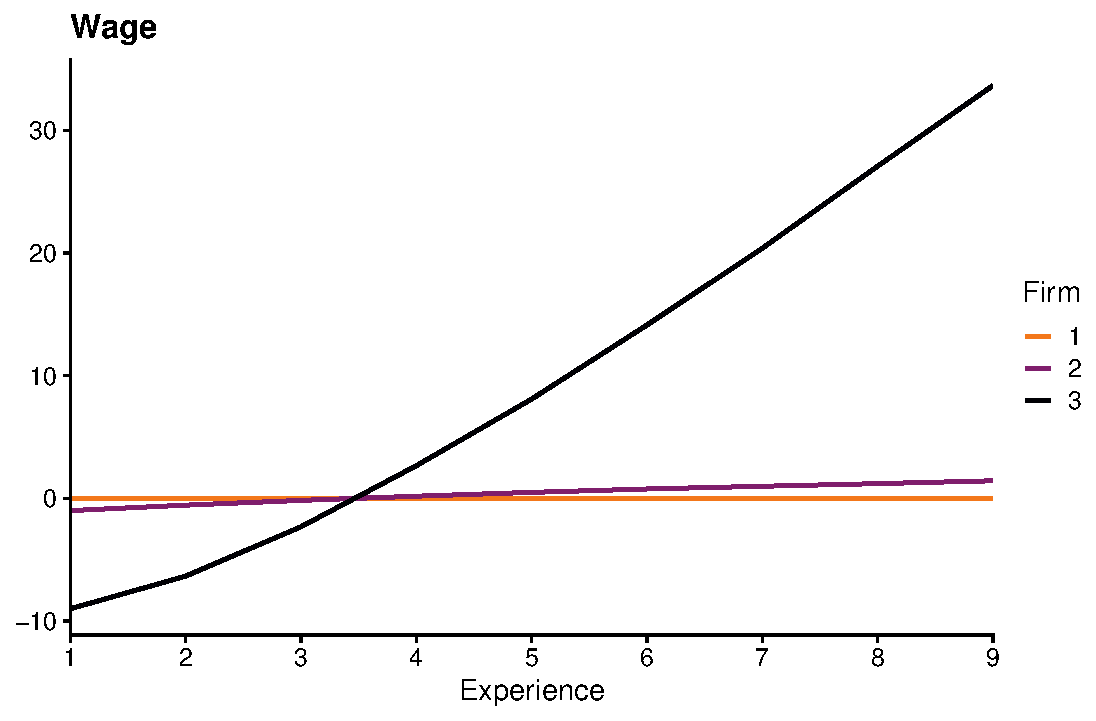
\includegraphics[width=0.5\textwidth]{DynamicWages.pdf}
}{%
  \caption{Wage Profiles}%
  \label{fig:earnings_profiles}%
}
\capbtabbox{%
  \begin{tabular}{lcc}
   \tabularnewline\midrule\midrule
   & TWFE &\\
   & Estimate & ATT\\
   \midrule
   Firm 2       & -0.5599$^{***}$ & 0.3\\
                       & (0.0429) & \\
   Firm 3       & -1.563 & 9.71\\
                       & (1.449) & \\
   \midrule \emph{Fixed} &  & \\
    \emph{effects} &  & \\
   Time                   & Yes& \\
   Worker              & Yes & \\
   \midrule
\end{tabular}
}{%
  \caption{Estimates}%
  \label{tab:dynamic_ests}%
}
\end{floatrow}
\end{figure}

% \begin{table}[]
%     \centering
%     \caption{Earnings Profiles}
%     \label{tab:TWFE}
%     \begin{tabular}{lcc}
%   \tabularnewline\midrule\midrule
%   & TWFE Estimate & ATT\\
%   \midrule
%   Firm 2       & -0.5599$^{***}$ & 0.3\\
%                       & (0.0429) & \\
%   Firm 3       & -1.563 & 9.71\\
%                       & (1.449) & \\
%   \midrule \emph{Fixed-effects} &  & \\
%   Time                   & Yes& \\
%   Worker              & Yes & \\
%   \midrule
% \end{tabular}
% \end{table}

The case of heterogeneous effects of continuous-valued covariates is a little strange. In \citet{callaway2021difference}, they describe their desired parameter when running differences-in-differences with a continuous treatment, the average causal response on the treated. They show that, with two-way fixed effects, this isn't identified if the groups receiving a small dose have a large treatment effect, while the groups receiving a large dose have a small treatment effect. In fact, even in a non-staggered setting, the TWFE estimate can be negative when all of the treatment effects are positive in this continuous case. But the point that's relevant here, which they don't discuss because they aren't interested in the fixed effects themselves, is that the fixed effects also do not represent any useful average in that case. % Table \ref{tablex} shows the estimated fixed effects in the case where all the true fixed effects are 0, and the high dose group gets a dose of 10 and a response of 1, while the low dose group gets a dose of 1 and has a response of 10.
This matters in the context of AKM because it is often estimated with time varying covariates like experience or tenure. If those enter linearly, the same issue can occur. This might be less interesting overall; I think it can be fixed by simply saturating those covariates (for example \citet{woodcock2015match} advocates a flexible tenure function with a dummy for each year, while \citet{lachowska2020sources} use a linear one).

I also find an issue in the case of heterogeneous effects of time on earnings, even with constant worker and firm effects, which in the differences-in-differences literature is a violation of the parallel trends assumption. But given the whole idea here, that any fixed effect can be thought of as a treatment, it seems natural to think about time heterogeneity, though identification will probably require imposing some structure on that heterogeneity. And when the treatment effects don't correspond to the ATT because of odd weighting, the fixed effects don't tend to correspond to the average fixed effects, something I hope I can prove formally.

Heterogeneous time effects are very natural in the context of earnings processes because age-earnings profiles are not linear. Table \ref{tab:TimeHet} shows an example where the earnings process is hump shaped in age ($Y_i = \alpha_f - (50 - \text{age}_i) ^ 2 + \varepsilon_i$), and workers at firm $1$ are younger than those at firm $0$. Worker effects are 0, and $\alpha_1 = 1$ and $\alpha_0 = 0$, so the ATT is $1$, but TWFE estimates a negative value of $-0.13$ (estimating an overly negative effect of aging on the younger workers at firm $1$).

\begin{table}[H]
    \centering
    \caption{Time Heterogeneity}
   \begin{tabular}{lc}
   \tabularnewline\midrule\midrule
   & Wages\\
   \midrule \emph{Variables} &  \\
   Firm 1       & -0.126\\
   Time 2        & -3.369\\
   \midrule \emph{Fixed effects} &  \\
   Worker              & Yes\\
   \midrule
\end{tabular}
    \label{tab:TimeHet}
\end{table}

Now, I implement the iterative estimator using the approach of \citet{sun2021estimating} on simulated data. I only am able to iterate the firm effects, because the worker effects don't fit nicely into the panel framework. The estimates in Figure \ref{fig:firmEffects} show $\alpha^10$, the results after 10 iterations of the firm effects (labeled SA, for Sun-Abraham). The iteration substantially improves the estimates, but they still are worse than TWFE. Figure \ref{fig:firmEffects} does show that TWFE is biased upwards in the presence of match effects and differential earnings profiles (firms 3--10 have steeper tenure-earnings profiles). Still, I am glad to show that I can simulate data with match effects, heterogeneous age-earnings and tenure-earnings profiles, and heterogenous firm sizes, and then output the ATT as I've set it up.

\begin{figure}[H]
    \centering
    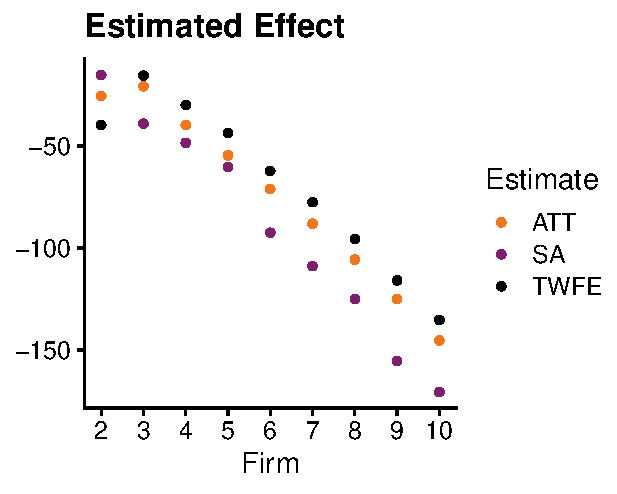
\includegraphics{FirmEffects.pdf}
    \caption{Firm Effect Simulations}
    \label{fig:firmEffects}
\end{figure}

\section{Empirical Application}

For an empirical application, I could compute a new estimator using matched employer-employee data and compare the results to existing estimates of the extent of assortative matching (\citealp{kline2020leave}; \citealp{bonhomme2022discretizing}), the role of firm effects in gender or racial inequality (\citealp{card2016bargaining}; \citealp{gerard2021assortative}), or inequality (\citealp{card2013workplace}, \citealp{song2019firming}, \citealp{wilmers2021consolidated}). This is probably the best approach for showcasing a new estimator; comparing it to existing implementations.

But I think there are some other interesting questions that can be answered with AKM, and particularly require care in estimation of firm effects, not just unbiased estimates of variance decompositions. Those questions are about endogenizing firm pay premia. Do firms pay high wages because they earn rents in the product market and workers are able to bargain for a share of those rents? Are pay premia chosen in response to local labor market competitiveness? Does pay dispersion emerge in equilibrium as in \citet{burdett1998wage}, where higher wage firms benefit from lower turnover and reduced vacancy posting time? Or does market power give employers scope to set wages far from the optimum and still survive \citep{dube2018monopsony}? Perhaps high-wage firms are simply unaware of the extent to which they could lower wages and retain their workers, like employers on M-Turk \citep{dube2020monopsony}.

As a start, I think it would be interesting to match estimated firm effects to vacancy data from Burning Glass and see how high-paying firms' experience in search and matching markets differs from low-paying firms: whether they receive more applications, whether they fill their vacancies more quickly, and possibly whether they choose higher worker effect workers (though at least in the U.S. I don't think it would be possible to match applications to worker effects due to privacy concerns). This would offer an empirical test of models of job search like \citet{burdett1998wage} and \citet{postel2002equilibrium} that would improve upon work that uses only realized matches to test those models like \citet{di2021ain}.

\newpage

\bibliography{bibfile}

\end{document}
